\documentclass[tikz, border=10pt]{standalone}
\usepackage[utf8]{inputenc}
% Note: To render Bengali text, use XeLaTeX and a font like Kalpurush if needed.
% For standard LaTeX, the text is provided as-is in the node.

\begin{document}
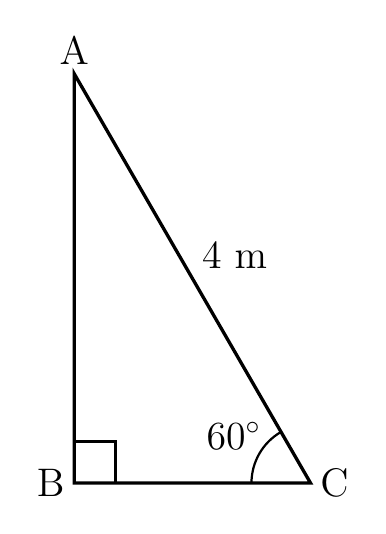
\begin{tikzpicture}[scale=1.5]
    % Define coordinates based on 60-degree trigonometry
    % If BC = 2, then AB = 2 * tan(60) = 2 * 1.732 = 3.464
    \coordinate (A) at (0, 3.464);
    \coordinate (B) at (0, 0);
    \coordinate (C) at (2, 0);

    % Draw the triangle with the requested very thick lines
    \draw[very thick] (A) -- (B) -- (C) -- cycle;

    % Draw the right angle symbol at vertex B
    \draw[very thick] (0, 0.35) -- (0.35, 0.35) -- (0.35, 0);

    % Draw the angle arc inside vertex C
    % The arc is drawn from the direction of B (180 deg) towards A (120 deg)
    \draw[thick] (1.5, 0) arc (180:120:0.5);
    
    % Label for the 60 degree angle
    \node at (1.35, 0.4) {\Large $60^\circ$};

    % Label for the hypotenuse (4 meters in Bengali)
    % Positioned near the midpoint of the hypotenuse AC
    \node[above right] at (1.0, 1.732) {\Large 4 m};

    % Labels for the vertices A, B, and C
    \node[above] at (A) {\Large A};
    \node[left] at (B) {\Large B};
    \node[right] at (C) {\Large C};

\end{tikzpicture}
\end{document}